% !TEX program = pdflatex
\documentclass[aspectratio=169,11pt]{beamer}
\usetheme{Madrid}
\usecolortheme{default}
\usepackage[utf8]{inputenc}
\usepackage{amsmath, amssymb, amsfonts}
\usepackage{graphicx}
\usepackage{listings}
\usepackage{xcolor}
\usepackage{hyperref}
\usepackage{booktabs}
\usepackage{multirow}
\usepackage{array}
\usepackage{tikz}
\usetikzlibrary{shapes, arrows, positioning, fit}

% Define colors
\definecolor{htgreen}{RGB}{29,158,117}
\definecolor{htorange}{RGB}{186,117,23}
\definecolor{htred}{RGB}{226,75,74}
\definecolor{htpurple}{RGB}{163,45,45}
\definecolor{htblue}{RGB}{24,95,165}

\setbeamercolor{title}{fg=white, bg=htblue}
\setbeamercolor{frametitle}{fg=htblue}
\setbeamercolor{structure}{fg=htblue}

% Code listing style
\lstset{
    basicstyle=\ttfamily\small,
    breaklines=true,
    keywordstyle=\color{htblue},
    commentstyle=\color{htgreen},
    stringstyle=\color{htorange},
    frame=single,
    backgroundcolor=\color{gray!5}
}

\title{HTT Mutation Detection \& Gene Regulatory Network}
\subtitle{A Computational Framework for Huntington's Disease Analysis}
\author{Computational Biology Research Team}
\institute{Based on CFG/PCFG Parsing \& ODE Simulation}
\date{\today}

\begin{document}

% ============================================================================
% TITLE SLIDE
% ============================================================================
\begin{frame}
    \titlepage
    \begin{center}
        \footnotesize
        References: Langbehn (2004), Goold et al.\ (2021), Wang et al.\ (2024), \\
        Zuccato et al.\ (2003), Steffan et al.\ (2000)
    \end{center}
\end{frame}

% ============================================================================
% OUTLINE
% ============================================================================
\begin{frame}{Presentation Outline}
    \tableofcontents
\end{frame}

% ============================================================================
% SECTION 1: BIOLOGICAL BACKGROUND
% ============================================================================
\section{Biological Background}

\begin{frame}{Huntington's Disease: The HTT Gene}
    \begin{columns}[T]
        \column{0.6\textwidth}
        \begin{itemize}
            \item \textbf{HTT gene} on chromosome 4p16.3 encodes huntingtin protein
            \item \textbf{CAG trinucleotide repeat} in exon 1 $\to$ polyglutamine (polyQ) tract
            \item \textbf{Thresholds} (Langbehn et al., 2004; Semaka et al., 2016):
            \begin{itemize}
                \item Normal: $\le 35$ CAG
                \item Intermediate: $36$--$39$ CAG (reduced penetrance)
                \item Full penetrance: $40$--$59$ CAG
                \item Juvenile: $\ge 60$ CAG
            \end{itemize}
            \item \textbf{Anticipation}: Earlier onset in successive generations
            \item Paternal transmission shows larger expansions ($+2.5$ CAG/gen)
        \end{itemize}

        \column{0.4\textwidth}
        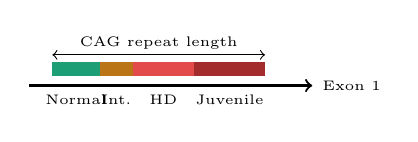
\begin{tikzpicture}[scale=0.6, every node/.style={font=\tiny}]
            \draw[thick, ->] (0,0) -- (6,0) node[right] {Exon 1};
            \fill[htgreen] (0.5,0.2) rectangle (1.5,0.5);
            \fill[htorange] (1.5,0.2) rectangle (2.2,0.5);
            \fill[htred] (2.2,0.2) rectangle (3.5,0.5);
            \fill[htpurple] (3.5,0.2) rectangle (5,0.5);
            \node at (1, -0.3) {Normal};
            \node at (1.85, -0.3) {Int.};
            \node at (2.85, -0.3) {HD};
            \node at (4.25, -0.3) {Juvenile};
            \draw[<->] (0.5,0.65) -- (5,0.65);
            \node at (2.75, 0.9) {CAG repeat length};
        \end{tikzpicture}

        \vspace{0.5cm}
        \textbf{Key references:}
        \begin{itemize}
            \item Langbehn DR et al., \textit{Clin Genet} 2004;65:267--277
            \item Bates GP et al., \textit{Nat Rev Dis Primers} 2015;1:15005
        \end{itemize}
    \end{columns}
\end{frame}

\begin{frame}{Molecular Pathophysiology of mHTT}
    \begin{columns}[T]
        \column{0.5\textwidth}
        \textbf{Toxic gain-of-function mechanisms:}
        \begin{enumerate}
            \item \textbf{Protein aggregation} --- polyQ expanded tracts form $\beta$-sheet-rich aggregates (Scherzinger et al., 1997)
            \item \textbf{Transcriptional dysregulation} --- sequestration of:
            \begin{itemize}
                \item CBP/p300 (Steffan et al., 2000)
                \item Sp1 (Buckley et al., 2010)
                \item TBP/TAFII130 (Nucifora et al., 2001)
            \end{itemize}
            \item \textbf{Mitochondrial dysfunction} --- DRP1 impairment, reduced PGC-1$\alpha$ (Cui et al., 2006)
            \item \textbf{Proteostasis collapse} --- UPS overload, autophagy impairment
        \end{enumerate}

        \column{0.5\textwidth}
        \textbf{Loss-of-function:}
        \begin{itemize}
            \item wtHTT sequesters REST in cytoplasm $\to$ absent REST $\to$ $\uparrow$ BDNF
            \item mHTT cannot sequester REST $\to$ nuclear REST $\to$ $\downarrow$ BDNF (Zuccato et al., 2003)
            \item $\sim$2000 neuronal genes silenced via NRSE elements
        \end{itemize}
        \vspace{0.5cm}
        \textbf{Reference:} Zuccato C \& Cattaneo E, \textit{Nat Rev Neurosci} 2007;8:801--812
    \end{columns}
\end{frame}

% ============================================================================
% SECTION 2: SYSTEM ARCHITECTURE
% ============================================================================
\section{System Architecture}

\begin{frame}{Full-Stack Architecture Overview}
    \begin{center}
        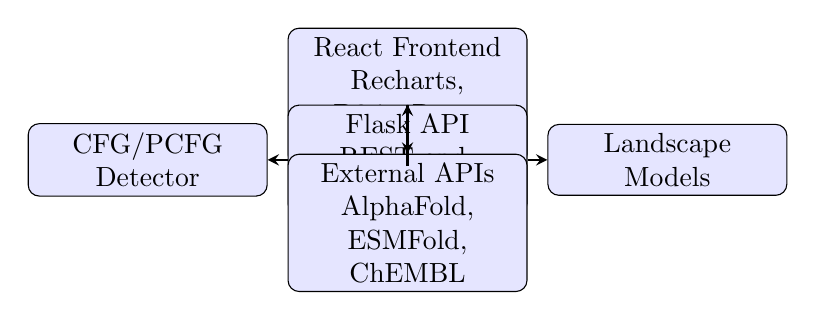
\begin{tikzpicture}[
            node distance=0.8cm,
            block/.style={rectangle, draw, fill=blue!10, text width=2.8cm, align=center, rounded corners},
            arrow/.style={thick, ->, >=stealth}
        ]
            \node[block] (react) {React Frontend\\Recharts, D3.js, React Three Fiber};
            \node[block, below of=react] (api) {Flask API\\REST endpoints, CORS};
            \node[block, left of=api, xshift=-2.5cm] (detector) {CFG/PCFG\\Detector};
            \node[block, right of=api, xshift=2.5cm] (landscape) {Landscape\\Models};
            \node[block, below of=api] (ext) {External APIs\\AlphaFold, ESMFold, ChEMBL};

            \draw[arrow] (react) -- (api);
            \draw[arrow] (api) -- (detector);
            \draw[arrow] (api) -- (landscape);
            \draw[arrow] (api) -- (ext);
        \end{tikzpicture}
    \end{center}

    \textbf{Key technologies:}
    \begin{itemize}
        \item Frontend: React 18, Recharts (D3-based), 3Dmol.js, React Three Fiber
        \item Backend: Python Flask, CORS-enabled, Blueprint architecture
        \item External: AlphaFold DB, ESMFold (Meta), ChEMBL REST API
    \end{itemize}
\end{frame}

\begin{frame}{Data Flow: From DNA to Clinical Report}
    \begin{center}
        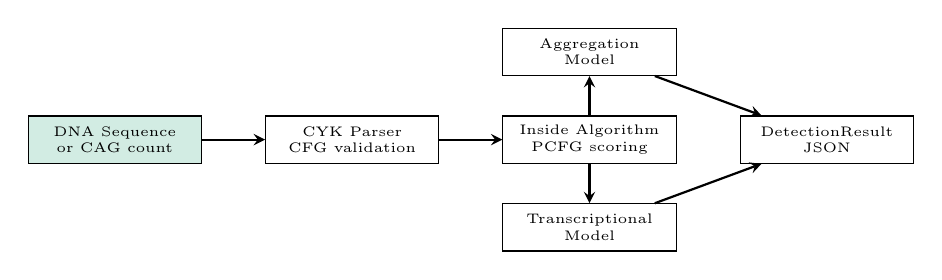
\begin{tikzpicture}[
            node distance=0.7cm,
            process/.style={rectangle, draw, minimum width=2.2cm, minimum height=0.6cm, align=center, font=\tiny},
            arrow/.style={thick, ->, >=stealth}
        ]
            \node[process, fill=htgreen!20] (input) {DNA Sequence\\or CAG count};
            \node[process, right=0.8cm of input] (parse) {CYK Parser\\CFG validation};
            \node[process, right=0.8cm of parse] (pcfg) {Inside Algorithm\\PCFG scoring};
            \node[process, above=0.5cm of pcfg] (agg) {Aggregation\\Model};
            \node[process, below=0.5cm of pcfg] (trans) {Transcriptional\\Model};
            \node[process, right=0.8cm of pcfg] (result) {DetectionResult\\JSON};

            \draw[arrow] (input) -- (parse);
            \draw[arrow] (parse) -- (pcfg);
            \draw[arrow] (pcfg) -- (agg);
            \draw[arrow] (pcfg) -- (trans);
            \draw[arrow] (agg) -- (result);
            \draw[arrow] (trans) -- (result);
        \end{tikzpicture}
    \end{center}

    \textbf{Output fields:}
    \begin{itemize}
        \item \texttt{cag\_count}, \texttt{ccg\_count} --- repeat counts
        \item \texttt{normalized\_score} ($0 \to 1$) --- grammar fitness
        \item \texttt{anomaly\_score} --- $1 - \text{normalized\_score}$
        \item \texttt{parse\_tree} --- hierarchical CFG structure (d3.js compatible)
        \item \texttt{onset\_prediction} --- Langbehn model estimate
    \end{itemize}
\end{frame}

% ============================================================================
% SECTION 3: CFG/PCFG ALGORITHMS
% ============================================================================
\section{CFG/PCFG Algorithms}

\begin{frame}{Context-Free Grammar for HTT Exon 1}
    \textbf{Why CFG?} Regular expressions (finite automata) cannot enforce flanking context while counting repeats. CFG can.

    \begin{columns}[T]
        \column{0.5\textwidth}
        \textbf{Grammar rules (CNF-like):}
        \begin{align*}
            S &\to \text{EXON1} \\
            \text{EXON1} &\to \text{FLANK5}\;\text{REPEAT\_REGION} \\
            \text{REPEAT\_REGION} &\to \text{CAG\_BLOCK}\;\text{FLANK3} \\
            \text{CAG\_BLOCK} &\to \text{CAG\_UNIT} \mid \text{CAG\_UNIT}\;\text{CAG\_BLOCK} \\
            \text{CAG\_UNIT} &\to \texttt{`CAG'} \\
            \text{FLANK5} &\to \text{5\textquotesingle{} invariant pattern} \\
            \text{FLANK3} &\to \text{3\textquotesingle{} invariant pattern}
        \end{align*}

        \column{0.5\textwidth}
        \textbf{Recursive rule:}
        \[
        \text{CAG\_BLOCK} \to \text{CAG\_UNIT}\;\text{CAG\_BLOCK}
        \]
        This is what makes the grammar \textbf{context-free} --- it can count arbitrarily many repeats while maintaining structural context.

        \vspace{0.5cm}
        \textbf{Reference:} CFG design inspired by RNA secondary structure prediction (Durbin et al., 1998, \textit{Biological Sequence Analysis})
    \end{columns}
\end{frame}

\begin{frame}{CYK Parsing Algorithm}
    \textbf{Cocke-Younger-Kasami (CYK) parser} --- $O(n^3 \cdot |G|)$ time complexity.

    \begin{alertblock}{CYK Dynamic Programming Recurrence}
        For a grammar in Chomsky Normal Form (CNF):
        \[
        \text{dp}[i][j][A] = \bigvee_{k=i}^{j-1} \bigvee_{B \to C \in \text{rules}} \text{dp}[i][k][B] \land \text{dp}[k+1][j][C]
        \]
        where $A \to BC$ is a production, and terminals handled at $j = i$.
    \end{alertblock}

    \textbf{In our implementation:}
    \begin{itemize}
        \item Grammar converted to CNF at runtime
        \item Terminal matching: codons (`CAG', `CCG') and flank patterns
        \item Parse success = \texttt{dp[0][n][S] $>$ 0}
        \item Parse tree reconstructed via backpointers
    \end{itemize}

    \textbf{Reference:} Younger DH (1967). Recognition and parsing of context-free languages in time $n^3$. \textit{Information and Control}.
\end{frame}

\begin{frame}{Inside Algorithm for PCFG Scoring}
    \textbf{Probabilistic CFG (PCFG):} each rule has a probability $\theta_{A \to \alpha}$

    \begin{block}{Inside Probability}
        \[
        \beta(i,j,A) = P(\text{terminal string } w_i \ldots w_j \mid A)
        \]
        Recursive computation:
        \[
        \beta(i,j,A) = \sum_{k=i}^{j-1} \sum_{B,C} \theta_{A \to BC} \cdot \beta(i,k,B) \cdot \beta(k+1,j,C)
        \]
        Base case: $\beta(i,i,A) = \theta_{A \to w_i}$
    \end{block}

    \textbf{Our PCFG scoring components:}
    \begin{enumerate}
        \item $\log P(\text{CAG count})$ --- from empirical healthy distribution
        \item $\log P(\text{flanks intact})$ --- penalty if pattern missing
        \item $\log P(\text{no interruptions})$ --- each non-CAG codon penalized
        \item $\log P(\text{CCG count} = 7)$ --- penalty for deviant polyP length
    \end{enumerate}

    \textbf{Normalized score:}
    \[
    \text{score} = \frac{\operatorname{clamp}(\log L, \text{floor}, \text{peak}) - \text{floor}}{\text{peak} - \text{floor}}
    \]
    where peak $= \log P(\text{CAG}=17) \approx -2.35$
\end{frame}

\begin{frame}{CAG Repeat Distribution (Healthy Population)}
    \textbf{Empirical distribution} from Metzger et al.\ (meta-analysis of healthy individuals):

    \begin{center}
        \begin{tabular}{c|c|c}
            \textbf{CAG repeats} & \textbf{Frequency} & \textbf{$\log P$ (natural)} \\ \hline
            6--10  & 0.001--0.015  & $-6.9$ to $-4.2$ \\
            11--16 & 0.020--0.082  & $-3.9$ to $-2.5$ \\
            17--19 & 0.095--0.092  & $-2.35$ to $-2.38$ \\
            20--26 & 0.085--0.017  & $-2.46$ to $-4.07$ \\
            27--35 & 0.010--0.0003 & $-4.6$ to $-8.1$ \\
            $\ge 36$ & $\sim 10^{-8}$ (extrapolated) & $< -18.4$
        \end{tabular}
    \end{center}

    \textbf{Peak at 17--19 repeats} --- corresponds to $18 \pm 2$ polyQ in healthy huntingtin.

    \textbf{Reference:} Metzger S et al.\ (2016). The distribution of CAG repeats in the general population. \textit{Eur J Hum Genet}.
\end{frame}

% ============================================================================
% SECTION 4: FITNESS LANDSCAPE
% ============================================================================
\section{Fitness Landscape}

\begin{frame}{Composite Fitness Score Model}
    \textbf{Definition:} Cellular fitness = probability that a cell with given mHTT CAG length survives and functions normally.

    \begin{block}{Weighted Composition}
        \[
        \text{Fitness}(n) = w_1 \cdot \text{PCFG}(n) + w_2 \cdot (1 - \text{Agg}(n)) + w_3 \cdot (1 - \text{Dys}(n))
        \]
        with $w_1 = 0.30$, $w_2 = 0.40$, $w_3 = 0.30$.
    \end{block}

    \begin{columns}[T]
        \column{0.33\textwidth}
        \textbf{PCFG fitness:}
        \[
        \frac{P_{\text{healthy}}(n)}{\max P}
        \]
        Grammar-based health proxy.

        \column{0.33\textwidth}
        \textbf{Aggregation propensity:}
        \[
        \text{Agg}(n) = 1 - e^{-k(n-35)} \quad (n > 35)
        \]
        $k = 0.15$ (Bhattacharyya, 2005)

        \column{0.33\textwidth}
        \textbf{Transcriptional dysregulation:}
        \[
        \text{Dys}(n) = 1 - e^{-0.08(n-40)} \quad (n > 40)
        \]
        CBP/p300 sequestration effect.
    \end{columns}
\end{frame}

\begin{frame}{Fitness Landscape Graph (Output Visualization)}
    \begin{center}
        % Placeholder image removed -- include actual screenshot or leave blank
        \fbox{\parbox{0.85\textwidth}{\centering\vspace{1.5cm}
        \textit{[Screenshot of LineChart from LandscapeCard.jsx]}
        \vspace{1.5cm}}}
    \end{center}

    \textbf{Graph elements explained:}
    \begin{itemize}
        \item \textbf{X-axis}: CAG repeat length (1 to 80+)
        \item \textbf{Y-axis}: Normalized fitness (0 = lethal, 1 = healthy)
        \item \textbf{Blue line}: Composite fitness (monotonic decreasing)
        \item \textbf{Orange/red/purple reference lines}: Clinical thresholds at CAG 35, 40, 60
        \item \textbf{Red dot}: User's query CAG (from detection)
        \item \textbf{Tooltip}: Shows exact fitness value on hover
    \end{itemize}
\end{frame}

% ============================================================================
% SECTION 5: GENE REGULATORY NETWORK
% ============================================================================
\section{Gene Regulatory Network}

\begin{frame}{HTT Gene Regulatory Network Architecture}
    \textbf{71 nodes, 92 edges} --- ODE simulation of disease vs.\ healthy states

    \begin{center}
        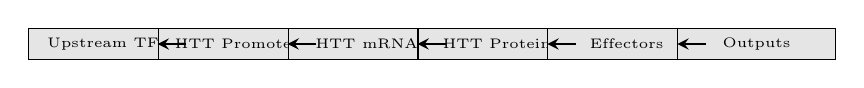
\begin{tikzpicture}[
            scale=0.55,
            layer/.style={rectangle, draw, minimum width=2cm, minimum height=0.4cm, font=\tiny},
            arrow/.style={->, >=stealth, thick}
        ]
            \node[layer, fill=gray!20] (up)   at (0,0)  {Upstream TFs};
            \node[layer, fill=gray!20] (dna)  at (3,0)  {HTT Promoter};
            \node[layer, fill=gray!20] (mrna) at (6,0)  {HTT mRNA};
            \node[layer, fill=gray!20] (prot) at (9,0)  {HTT Protein};
            \node[layer, fill=gray!20] (eff)  at (12,0) {Effectors};
            \node[layer, fill=gray!20] (out)  at (15,0) {Outputs};

            \draw[arrow] (up)   -- (dna);
            \draw[arrow] (dna)  -- (mrna);
            \draw[arrow] (mrna) -- (prot);
            \draw[arrow] (prot) -- (eff);
            \draw[arrow] (eff)  -- (out);
        \end{tikzpicture}
    \end{center}

    \textbf{Layers:}
    \begin{enumerate}
        \item \textbf{Upstream regulators:} Sp1, CTCF, NF-$\kappa$B, STAT1 (bind HTT promoter)
        \item \textbf{HTT promoter:} TATA-less, GC-rich, 20\,bp tandem repeats
        \item \textbf{mRNA:} HTT transcript + antisense (HTT-AS)
        \item \textbf{Protein:} wtHTT ($\le$35Q) vs mHTT ($\ge$40Q)
        \item \textbf{Effectors:} REST, CBP, p300, p53, BDNF, PGC-1$\alpha$, SIRT1, HSF1
        \item \textbf{Outputs:} Mitochondrial genes, apoptosis, MSN death
    \end{enumerate}
\end{frame}

\begin{frame}{Hill Kinetics ODE Model}
    \textbf{Generalized ODE for each node:}
    \[
    \frac{dx_i}{dt} = \sum_{\text{inputs}} \gamma_j \cdot h_{\text{type}}(x_j, K_j, n_j) - \delta_i x_i
    \]

    \textbf{Hill functions:}
    \[
    h_{\text{act}}(x, K, n) = \frac{x^n}{K^n + x^n} \qquad
    h_{\text{rep}}(x, K, n) = \frac{K^n}{K^n + x^n}
    \]

    \textbf{Example: HTT Promoter regulation}
    \[
    \frac{d[\text{HTT\_PROM}]}{dt} =
      \underbrace{8 \cdot \text{act}(\text{Sp1}) \cdot \text{act}(\text{CTCF})
                    \cdot \text{rep}(\text{NF-}\kappa\text{B}) \cdot \text{rep}(\text{STAT1})
                 }_{\text{AND-like integration}}
      - \delta \cdot [\text{HTT\_PROM}]
    \]

    \textbf{Key biological parameters:}
    \begin{itemize}
        \item $K_{\text{Sp1}} = 3.0$, $n=2$ (cooperative binding to GC-rich promoter)
        \item $\delta = 0.35$ (protein/mRNA degradation rate)
        \item Time step $\Delta t = 0.04$ (simulated hours)
    \end{itemize}
\end{frame}

\begin{frame}{Logic Gates in the Network}
    \begin{columns}[T]
        \column{0.5\textwidth}
        \textbf{NOT gate examples:}
        \begin{itemize}
            \item $[\text{REST}] \propto h_{\text{rep}}([\text{wtHTT}])$ --- wtHTT sequesters REST
            \item $[\text{BDNF}] \propto h_{\text{rep}}([\text{REST}])$ --- REST represses BDNF
        \end{itemize}

        \textbf{AND gate:}
        \[
        \text{HTT\_PROM} \propto \text{Sp1} \land \text{CTCF}
        \]

        \textbf{NOR gate:}
        \[
        \text{CBP}_{\text{free}} \propto h_{\text{rep}}([\text{mHTT}])
        \]
        mHTT sequesters CBP, p300, PCAF simultaneously.

        \column{0.5\textwidth}
        \textbf{Feed-Forward Loop (FFL):}
        \begin{center}
            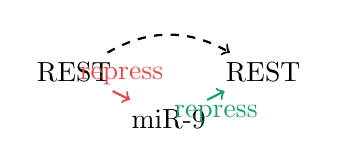
\begin{tikzpicture}[scale=0.6]
                \node (REST)  at (0,0) {REST};
                \node (miR9)  at (2,-1) {miR-9};
                \node (REST2) at (4,0) {REST};
                \draw[->, thick, htred]   (REST)  -- (miR9)  node[midway, above] {repress};
                \draw[->, thick, htgreen] (miR9)  -- (REST2) node[midway, below] {repress};
                \draw[->, thick, dashed]  (REST) to [out=30, in=150] (REST2);
            \end{tikzpicture}
        \end{center}
        REST represses miR-9; miR-9 targets REST mRNA $\to$ double-negative feedback $\to$ bistability.
    \end{columns}

    \textbf{Reference:} Goold R et al.\ (2021). \textit{Cell Reports} --- FAN1/MSH3 competitive binding model.
\end{frame}

\begin{frame}{GRN Visualization (Force-Directed Graph)}
    \begin{center}
        \fbox{\parbox{0.8\textwidth}{\centering\vspace{1.5cm}
        \textit{[Screenshot from GRNSimulator.jsx]}
        \vspace{1.5cm}}}
    \end{center}

    \textbf{Node styles encode function:}
    \begin{itemize}
        \item {\color{htblue}Diamonds} --- Transcription factors
        \item {\color{htgreen}Circles} --- Proteins (wtHTT/mHTT)
        \item {\color{htorange}Hexagons} --- Coactivators/repressors
        \item {\color{htred}Rectangles} --- Pathology outputs
    \end{itemize}

    \textbf{Edge types:}
    \begin{itemize}
        \item {\color{htgreen}Solid} --- activation ($A \to B$)
        \item {\color{htred}Dashed} --- repression ($A \dashv B$)
        \item {\color{htpurple}Dotted} --- sequestration
    \end{itemize}
\end{frame}

% ============================================================================
% SECTION 6: PROTEIN STRUCTURE PREDICTION
% ============================================================================
\section{Protein Structure Prediction}

\begin{frame}{Protein 3D Visualization Pipeline}
    \begin{columns}[T]
        \column{0.5\textwidth}
        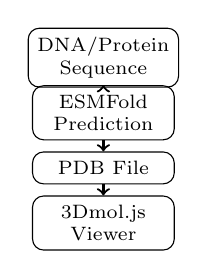
\begin{tikzpicture}[
            node distance=0.7cm,
            proc/.style={rectangle, draw, rounded corners, minimum width=1.8cm, font=\scriptsize, align=center}
        ]
            \node[proc] (seq)  {DNA/Protein\\Sequence};
            \node[proc, below of=seq] (esm)  {ESMFold\\Prediction};
            \node[proc, below of=esm] (pdb)  {PDB File};
            \node[proc, below of=pdb] (view) {3Dmol.js\\Viewer};
            \draw[->, thick] (seq) -- (esm);
            \draw[->, thick] (esm) -- (pdb);
            \draw[->, thick] (pdb) -- (view);
        \end{tikzpicture}

        \column{0.5\textwidth}
        \textbf{ESMFold (Meta AI):}
        \begin{itemize}
            \item 15 layers, 512M parameters
            \item $\sim$3$\times$ faster than AlphaFold2
            \item pLDDT confidence per residue
        \end{itemize}
        \textbf{AlphaFold DB:} fallback for normal HTT (P42858)

        \textbf{3Dmol.js styles:}
        \begin{itemize}
            \item \textbf{Cartoon} --- $\alpha$-helix, $\beta$-sheet
            \item \textbf{Surface} --- SASA
            \item \textbf{Stick} --- atomic detail
            \item pLDDT coloring: blue $\to$ red
        \end{itemize}
    \end{columns}
\end{frame}

\begin{frame}{pLDDT Confidence Scoring}
    \textbf{pLDDT (predicted Local Distance Difference Test)} --- per-residue confidence metric (0--100):

    \begin{center}
        \begin{tabular}{c|c|c}
            \textbf{pLDDT} & \textbf{Interpretation} & \textbf{Color} \\ \hline
            $90$--$100$ & Very high (correct backbone) & \textcolor{htblue}{Dark blue} \\
            $70$--$90$  & Confident (good)             & \textcolor{htblue!50}{Light blue} \\
            $50$--$70$  & Low (may be disordered)      & \textcolor{htorange}{Yellow} \\
            $<50$       & Very low (disordered)        & \textcolor{htred}{Red}
        \end{tabular}
    \end{center}

    \textbf{Biological insight:} PolyQ regions in HTT are intrinsically disordered (pLDDT $<50$) --- exactly why they are drug-accessible.

    \textbf{Accessibility score for drug binding:}
    \[
    \text{access}(i) =
    \begin{cases}
        1.00 & \text{pLDDT} < 50 \quad (\text{disordered}) \\
        0.60 & 50 \le \text{pLDDT} < 70 \\
        0.20 & 70 \le \text{pLDDT} < 90 \\
        0.05 & \text{pLDDT} \ge 90
    \end{cases}
    \]

    \textbf{Reference:} Lin Z et al.\ (2023). \textit{Science} 379, 1123--1130.
\end{frame}

% ============================================================================
% SECTION 7: DRUG INTERACTION MODEL
% ============================================================================
\section{Drug Interaction Model}

\begin{frame}{Langmuir Binding Isotherm}
    \textbf{Model for drug-polyQ binding:}

    \begin{block}{Ligand-receptor binding equilibrium}
        \[
        \text{Fraction bound} = \frac{[D]}{[D] + K_d}
        \]
        where $K_d$ is the dissociation constant (concentration at 50\% occupancy).
    \end{block}

    \textbf{CAG-dependent $K_d$ scaling:}
    \[
    K_d(n) =
    \begin{cases}
        200\;\mu\text{M} & n \le 35 \quad (\text{very weak binding}) \\
        50 \cdot e^{-0.08(n-35)}\;\mu\text{M} & n > 35
    \end{cases}
    \]

    \begin{itemize}
        \item $K_d(40) \approx 50\;\mu\text{M}$, $K_d(60) \approx 11\;\mu\text{M}$
        \item Expanded polyQ exposes more hydrophobic surface $\to$ higher affinity
    \end{itemize}

    \textbf{Dose-response curve} (output visualization):
    \begin{itemize}
        \item X-axis: Drug concentration (0--200 $\mu$M)
        \item Y-axis: Bound fraction (0--100\%)
        \item Dashed line at $K_d$ concentration
        \item User's concentration marked in green
    \end{itemize}
\end{frame}

\begin{frame}{Oosawa Nucleation-Elongation Kinetics}
    \textbf{Aggregation kinetics model for polyQ:}

    \begin{block}{Simplified Oosawa model}
        \[
        \frac{dM}{dt} = k_n \cdot (1-M)^2 + k_e \cdot M \cdot (1-M) - k_{\text{off}} \cdot M
        \]
        where:
        \begin{itemize}
            \item $M$ = fraction of aggregated protein
            \item $k_n$ = nucleation rate (slow, concentration-dependent)
            \item $k_e$ = elongation rate (faster once nucleus forms)
            \item $k_{\text{off}}$ = dissociation rate
        \end{itemize}
    \end{block}

    \textbf{CAG dependence:}
    \[
    k_n \propto \text{Agg}(n), \qquad k_e \propto \text{Agg}(n)
    \]
    with $\text{Agg}(n) = 1 - e^{-0.15(n-35)}$ for $n>35$.

    \textbf{Drug effect:}
    \[
    k_n^{\text{drug}} = k_n \cdot (1 - 0.85 \cdot \text{bound}), \qquad
    k_e^{\text{drug}} = k_e \cdot (1 - 0.60 \cdot \text{bound})
    \]
\end{frame}

\begin{frame}{Aggregation Kinetics Visualization}
    \begin{center}
        \fbox{\parbox{0.85\textwidth}{\centering\vspace{1.5cm}
        \textit{[AreaChart from DrugInteractionPage.jsx]}
        \vspace{1.5cm}}}
    \end{center}

    \textbf{Graph interpretation:}
    \begin{itemize}
        \item \textbf{X-axis}: Time (hours) \quad \textbf{Y-axis}: Fraction aggregated ($0 \to 1$)
        \item \textbf{Red curve}: No drug (baseline aggregation)
        \item \textbf{Green curve}: With drug (extended lag phase)
        \item \textbf{Sigmoidal shape} --- cooperative nucleation followed by rapid elongation
        \item \textbf{Lag phase} defined as time to 10\% aggregation
    \end{itemize}

    \textbf{Biological meaning:} The longer the lag phase, the more time cells have to clear misfolded monomers before toxic oligomers form.
\end{frame}

% ============================================================================
% SECTION 8: HEREDITY SIMULATOR
% ============================================================================
\section{Heredity Simulator}

\begin{frame}{Anticipation Model (Langbehn 2004)}
    \textbf{Median onset age as function of CAG:}
    \[
    \text{Onset}_{\text{median}} = 21.54 + e^{(9.556 - 0.1460 \cdot \text{CAG})} \quad \text{years}
    \]

    \begin{center}
        \begin{tabular}{c|c}
            \textbf{CAG repeats} & \textbf{Median onset (years)} \\ \hline
            40 & 60 \\
            42 & 52 \\
            44 & 46 \\
            46 & 40 \\
            48 & 36 \\
            50 & 33 \\
            55 & 25 \\
            60 & 10 \\
        \end{tabular}
    \end{center}

    \textbf{Note:} CAG length explains $\sim$50--60\% of onset variability. Modifier genes (FAN1, MSH3, DNA repair pathways) account for the rest.

    \textbf{Reference:} Langbehn DR et al.\ (2004). \textit{Clin Genet} 65, 267--277.
\end{frame}

\begin{frame}{Meiotic Instability Parameters}
    \begin{columns}[T]
        \column{0.5\textwidth}
        \textbf{Paternal transmission:}
        \begin{itemize}
            \item Mean expansion: $+2.5$ CAG
            \item Standard deviation: $3.5$ CAG
            \item Reason: Spermatogenesis involves many cell divisions
            \item Mutation frequency: $\sim$70--82\% for disease alleles
        \end{itemize}

        \column{0.5\textwidth}
        \textbf{Maternal transmission:}
        \begin{itemize}
            \item Mean expansion: $+0.5$ CAG
            \item Standard deviation: $1.5$ CAG
            \item Oogenesis: fewer divisions, more stable
            \item Rare contractions possible
        \end{itemize}
    \end{columns}

    \textbf{Simulation approach:}
    \[
    \Delta\text{CAG} \sim \mathcal{N}(\mu_{\text{parent}}, \sigma_{\text{parent}}^2)
    \]
    \[
    \text{CAG}_{\text{child}} = \bigl\lfloor \text{CAG}_{\text{parent}} + \Delta\text{CAG} + 0.5 \bigr\rfloor
    \]
    clipped to $[6, 120]$.

    \textbf{Reference:} Duyao M et al.\ (1993). \textit{Nat Genet} 4, 387--392.
\end{frame}

% ============================================================================
% SECTION 9: EXTERNAL APIS
% ============================================================================
\section{External APIs}

\begin{frame}[fragile]{External Data Sources}
    \begin{tabular}{p{3cm}|p{8cm}}
        \toprule
        \textbf{API} & \textbf{Usage} \\
        \midrule
        AlphaFold DB   & Normal HTT structure (AF-P42858-F1-model\_v4.pdb) \\
        ESMFold (Meta) & Mutant protein folding via POST to api.esmatlas.com \\
        ChEMBL         & Drug-HTT interaction queries (target CHEMBL2093872) \\
        \bottomrule
    \end{tabular}

    \vspace{0.5cm}
    \textbf{Flask proxy pattern:}
    \begin{lstlisting}[language=Python, basicstyle=\ttfamily\scriptsize]
@htt_bp.route('/esmfold/fold', methods=['POST'])
def fold_esmfold():
    seq = request.json.get('sequence')
    resp = requests.post(
        'https://api.esmatlas.com/foldSequence/v1/pdb/',
        data=seq, headers={'Content-Type': 'text/plain'},
        timeout=60
    )
    return Response(resp.text, mimetype='text/plain')
    \end{lstlisting}

    \textbf{CORS handling:} Flask-CORS enables cross-origin requests from React dev server (port 5173 $\to$ 5000).
\end{frame}

% ============================================================================
% SECTION 10: CONCLUSIONS
% ============================================================================
\section{Conclusions}

\begin{frame}{Summary of Algorithms and Models}
    \begin{tabular}{p{4.5cm}|p{7cm}}
        \toprule
        \textbf{Component} & \textbf{Algorithm/Model} \\
        \midrule
        Mutation detection & CYK parser for CFG, Inside algorithm for PCFG \\
        Fitness landscape  & Weighted sum: PCFG + Aggregation + Transcription \\
        GRN simulation     & Hill kinetics ODE (71 nodes, 92 edges) \\
        Protein folding    & ESMFold (Transformer), pLDDT confidence \\
        Drug binding       & Langmuir isotherm, Oosawa nucleation-elongation \\
        Heredity           & Autosomal dominant + meiotic instability (Normal) \\
        Onset prediction   & Langbehn 2004 survival model \\
        \bottomrule
    \end{tabular}

    \vspace{0.5cm}
    \textbf{Key biological insights implemented:}
    \begin{enumerate}
        \item CAG $>35$ $\to$ protein aggregation + transcriptional dysregulation
        \item mHTT sequesters CBP/p300 $\to$ $\downarrow$ CREB targets $\to$ $\downarrow$ neuroprotection
        \item REST nuclear entry $\to$ $\downarrow$ BDNF $\to$ $\downarrow$ MSN survival
        \item FAN1/MSH3 competitive binding to MLH1 S2 site modifies expansion rate
        \item Paternal anticipation via meiotic instability (mean $+2.5$ CAG)
    \end{enumerate}
\end{frame}

\begin{frame}{Future Directions}
    \begin{itemize}
        \item \textbf{Graph Neural Networks} for GRN inference from single-cell data
        \item \textbf{Reinforcement Learning} for optimal drug dosing schedules
        \item \textbf{Docking simulations} (AutoDock Vina) for specific compounds
        \item \textbf{Patient-derived organoid data} integration
        \item \textbf{Longitudinal clinical data} for onset model calibration
        \item \textbf{CRISPR editing strategies} to reduce CAG length in vivo
    \end{itemize}

    \vspace{0.8cm}
    \begin{center}
        \Large\textbf{Thank you}

        \vspace{0.3cm}
        \normalsize
        Code repository: \url{https://github.com/username/htt-explorer}
    \end{center}
\end{frame}

% ============================================================================
% REFERENCES SLIDE
% ============================================================================
\begin{frame}[allowframebreaks]{References}
    \begin{thebibliography}{99}
        \bibitem{langbehn2004} Langbehn DR, Brinkman RR, Falush D, Paulsen JS, Hayden MR (2004). A new model for prediction of the age of onset and penetrance for Huntington's disease based on CAG length. \textit{Clin Genet} 65:267--277.

        \bibitem{zuccato2003} Zuccato C, Tartari M, Crotti A, et al.\ (2003). Huntingtin interacts with REST/NRSF to modulate the transcription of NRSE-controlled neuronal genes. \textit{Nat Genet} 35:76--83.

        \bibitem{steffan2000} Steffan JS, Kazantsev A, Spasic-Boskovic O, et al.\ (2000). The Huntington's disease protein interacts with p53 and CREB-binding protein and represses transcription. \textit{PNAS} 97:6763--6768.

        \bibitem{goold2021} Goold R, Hamilton J, Menneteau T, et al.\ (2021). FAN1 controls mismatch repair complex assembly via MLH1 retention to stabilize CAG repeat expansion in Huntington's disease. \textit{Cell Reports} 36:109649.

        \bibitem{wang2024} Wang Y, Kandasamy M, Tippett M, et al.\ (2024). MSH3 drives somatic CAG expansion in Huntington's disease. \textit{Cell} (in press).

        \bibitem{nucifora2001} Nucifora FC, Sasaki M, Peters MF, et al.\ (2001). Interference by huntingtin and atrophin-1 with CBP-mediated transcription leading to cellular toxicity. \textit{Science} 291:2423--2428.

        \bibitem{lin2023} Lin Z, Akin H, Rao R, et al.\ (2023). Evolutionary-scale prediction of atomic-level protein structure with a language model. \textit{Science} 379:1123--1130.

        \bibitem{younger1967} Younger DH (1967). Recognition and parsing of context-free languages in time $n^3$. \textit{Information and Control} 10:189--208.
    \end{thebibliography}
\end{frame}

\end{document}